\documentclass{sigchi}

% Use this command to override the default ACM copyright statement (e.g. for preprints). 
% Consult the conference website for the camera-ready copyright statement.


%% EXAMPLE BEGIN -- HOW TO OVERRIDE THE DEFAULT COPYRIGHT STRIP -- (July 22, 2013 - Paul Baumann)
% \toappear{Permission to make digital or hard copies of all or part of this work for personal or classroom use is 	granted without fee provided that copies are not made or distributed for profit or commercial advantage and that copies bear this notice and the full citation on the first page. Copyrights for components of this work owned by others than ACM must be honored. Abstracting with credit is permitted. To copy otherwise, or republish, to post on servers or to redistribute to lists, requires prior specific permission and/or a fee. Request permissions from permissions@acm.org. \\
% {\emph{CHI'14}}, April 26--May 1, 2014, Toronto, Canada. \\
% Copyright \copyright~2014 ACM ISBN/14/04...\$15.00. \\
% DOI string from ACM form confirmation}
%% EXAMPLE END -- HOW TO OVERRIDE THE DEFAULT COPYRIGHT STRIP -- (July 22, 2013 - Paul Baumann)


% Arabic page numbers for submission. 
% Remove this line to eliminate page numbers for the camera ready copy
% \pagenumbering{arabic}


% Load basic packages
\usepackage{balance}  % to better equalize the last page
\usepackage{graphics} % for EPS, load graphicx instead
\usepackage{times}    % comment if you want LaTeX's default font
\usepackage{url}      % llt: nicely formatted URLs
\usepackage{tabulary}

% llt: Define a global style for URLs, rather that the default one
\makeatletter
\def\url@leostyle{%
  \@ifundefined{selectfont}{\def\UrlFont{\sf}}{\def\UrlFont{\small\bf\ttfamily}}}
\makeatother
\urlstyle{leo}


% To make various LaTeX processors do the right thing with page size.
\def\pprw{8.5in}
\def\pprh{11in}
\special{papersize=\pprw,\pprh}
\setlength{\paperwidth}{\pprw}
\setlength{\paperheight}{\pprh}
\setlength{\pdfpagewidth}{\pprw}
\setlength{\pdfpageheight}{\pprh}

% Make sure hyperref comes last of your loaded packages, 
% to give it a fighting chance of not being over-written, 
% since its job is to redefine many LaTeX commands.
\usepackage[pdftex]{hyperref}
\hypersetup{
pdftitle={SIGCHI Conference Proceedings Format},
pdfauthor={LaTeX},
pdfkeywords={SIGCHI, proceedings, archival format},
bookmarksnumbered,
pdfstartview={FitH},
colorlinks,
citecolor=black,
filecolor=black,
linkcolor=black,
urlcolor=black,
breaklinks=true,
}

% create a shortcut to typeset table headings
\newcommand\tabhead[1]{\small\textbf{#1}}


% End of preamble. Here it comes the document.
\begin{document}

\title{Visualizing the Statewide Impact of a Revenue-Neutral Carbon Tax}

\numberofauthors{4}
\author{
  \alignauthor Justin Bare\\
    \affaddr{University of Washington}\\
    \affaddr{Seattle, WA, USA}\\
    \email{jbare@cs.washington.edu}\\
    \affaddr{}
  \alignauthor Nandita Anand\\
      \affaddr{University of Washington}\\
      \affaddr{Seattle, WA, USA}\\
      \email{email@email.email}\\
      \affaddr{}
  \alignauthor Aditya Kaul\\
      \affaddr{University of Washington}\\
      \affaddr{Seattle, WA, USA}\\
      \email{email@email.email}\\
      \affaddr{}
  \alignauthor Richard Li\\
      \affaddr{University of Washington}\\
      \affaddr{Seattle, WA, USA}\\
      \email{email@email.email}\\
      \affaddr{}
}

\maketitle

\begin{abstract}
Abstract goes here
\end{abstract}

\keywords{
	Value Sensitive Design; politics
}

%\category{H.5.m.}{Information Interfaces and Presentation (e.g. HCI)}{Miscellaneous}

%See: \url{http://www.acm.org/about/class/1998/}
%for more information and the full list of ACM classifiers
%and descriptors. \newline
%\textcolor{red}{Optional section to be included in your final version, 
%but strongly encouraged. On the submission page only the classifiers’ 
%letter-number combination will need to be entered.}

\section{Introduction}

Intro goes here

The Carbon Washington revenue-neutral carbon tax proposal is composed of four main parts: 
\begin{enumerate}
\item reducing the state sales tax,
\item funding a tax rebate for low income households,
\item eliminating a business tax for manufacturers,
\item and instituting a tax on fossil fuels.
\end{enumerate}
``Revenue-neutral'' means that the total amount that the Washington state government raises 
from taxes every year will not change significantly as a result of this policy. The revenue 
reductions (1 and 3 above) and the additional spending (2) will be balanced by the new 
revenue source of the tax on fossil fuels (4).  

\section{Related Work}
Related work goes here

\subsection{Subsection}



\section{Methods}
Methods goes here
\begin{figure*}[t]
\centering
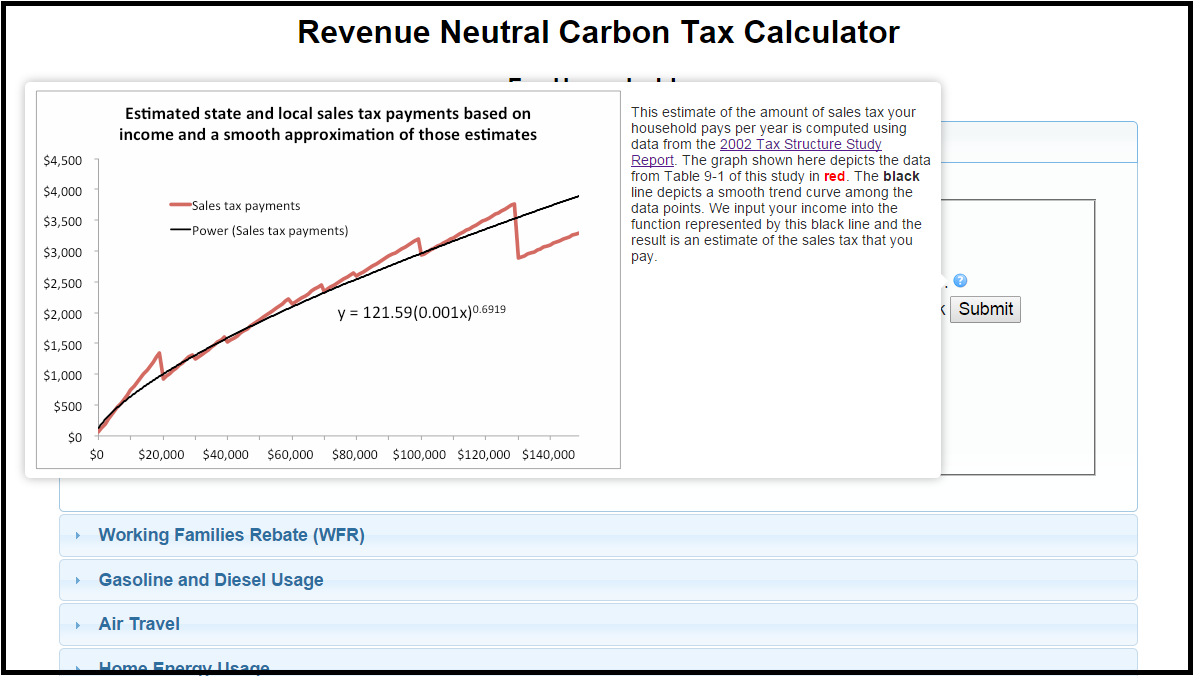
\includegraphics[width=0.9\textwidth]{toolTipDemo}
\caption{Tooltip that explains how a user's sales tax is estimated from their income in order to support the value of transparency.}
\label{fig:tooltip}
\end{figure*}

\section{Results}
Results goes here

\section{Discussion}
Discussion goes here

\section{Future Work}
Future work goes here
\begin{itemize}
\item A 
\item B
\item C

\end{itemize}

\subsection{Empirical Investigation}
Describe evaluation process

\section{Acknowledgments}

This material is based upon work supported by the National Science Foundation
Graduate Research Fellowship Program under Grant No. DGE-1256082.

% Balancing columns in a ref list is a bit of a pain because you
% either use a hack like flushend or balance, or manually insert
% a column break.  http://www.tex.ac.uk/cgi-bin/texfaq2html?label=balance
% multicols doesn't work because we're already in two-column mode,
% and flushend isn't awesome, so I choose balance.  See this
% for more info: http://cs.brown.edu/system/software/latex/doc/balance.pdf
%
% Note that in a perfect world balance wants to be in the first
% column of the last page.
%
% If balance doesn't work for you, you can remove that and
% hard-code a column break into the bbl file right before you
% submit:
%
% http://stackoverflow.com/questions/2149854/how-to-manually-equalize-columns-
% in-an-ieee-paper-if-using-bibtex
%
% Or, just remove \balance and give up on balancing the last page.
%
\balance

% REFERENCES FORMAT
% References must be the same font size as other body text.
\bibliographystyle{acm-sigchi}
\bibliography{sample}
\end{document}
